% ****** Start of file apssamp.tex ******
%
%   This file is part of the APS files in the REVTeX 4.1 distribution.
%   Version 4.1r of REVTeX, August 2010
%
%   Copyright (c) 2009, 2010 The American Physical Society.
%
%   See the REVTeX 4 README file for restrictions and more information.
%
% TeX'ing this file requires that you have AMS-LaTeX 2.0 installed
% as well as the rest of the prerequisites for REVTeX 4.1
%
% See the REVTeX 4 README file
% It also requires running BibTeX. The commands are as follows:
%
%  1)  latex apssamp.tex
%  2)  bibtex apssamp
%  3)  latex apssamp.tex
%  4)  latex apssamp.tex
%
%\documentclass[11pt]{article}
\documentclass[aps,prb,preprint,superscriptaddress]{revtex4-1}
%\documentclass[%
% reprint,
%%superscriptaddress,
%%groupedaddress,
%%unsortedaddress,
%%runinaddress,
%%frontmatterverbose, 
%%preprint,
%%showpacs,preprintnumbers,
%%nofootinbib,
%%nobibnotes,
%%bibnotes,
% amsmath,amssymb,
% aps,
%%pra,
% prb,
%%rmp,
%%prstab,
%%prstper,
%%floatfix,
%]{revtex4-1}
\usepackage{CJK}
\usepackage[T1]{fontenc}
\usepackage[utf8]{inputenc} % set input encoding (not needed with XeLaTeX)
\usepackage{setspace}
%\doublespacing

%%%% Examples of Article customizations
%% These packages are optional, depending whether you want the features they provide.
%% See the LaTeX Companion or other references for full information.
%
%%%% PAGE DIMENSIONS
\usepackage[margin=0.7in]{geometry} % to change the page dimensions
%%\geometry{a4paper} % or letterpaper (US) or a5paper or....
%% \geometry{margins=2in} % for example, change the margins to 2 inches all round
%% \geometry{landscape} % set up the page for landscape
%%   read geometry.pdf for detailed page layout information
%%\usepackage{amssymb,amsmath}
%\usepackage{graphicx} % support the \includegraphics command and options
%\usepackage[justification=justified,singlelinecheck=false,format=plain]{caption}
%\usepackage[justification=justified,singlelinecheck=false]{subcaption}
\usepackage{gensymb}
%
%% \usepackage[parfill]{parskip} % Activate to begin paragraphs with an empty line rather than an indent
%
%%%% PACKAGES
%%\usepackage{booktabs} % for much better looking tables
%\usepackage{array} % for better arrays (eg matrices) in maths
%%\usepackage{paralist} % very flexible & customisable lists (eg. enumerate/itemize, etc.)
%\usepackage{verbatim} % adds environment for commenting out blocks of text & for better verbatim
%%\usepackage{relsize} 
%\newcommand{\subscript}[1]{\raisebox{-0.25em}{\smaller #1}} 
%%\usepackage{subfig} % make it possible to include more than one captioned figure/table in a single float
%% These packages are all incorporated in the memoir class to one degree or another...
%
%%%% HEADERS & FOOTERS
%%\usepackage{fancyhdr} % This should be set AFTER setting up the page geometry
%%\pagestyle{fancy} % options: empty , plain , fancy
%%\renewcommand{\headrulewidth}{0pt} % customise the layout...
%%\lhead{}\chead{}\rhead{}
%%\lfoot{}\cfoot{\thepage}\rfoot{}
%
%%%% SECTION TITLE APPEARANCE
%%\usepackage{sectsty}
%%\allsectionsfont{\sffamily\mdseries\upshape} % (See the fntguide.pdf for font help)
%% (This matches ConTeXt defaults)
%
%%%% ToC (table of contents) APPEARANCE
%%\usepackage[nottoc,notlof,notlot]{tocbibind} % Put the bibliography in the ToC
%%\usepackage[titles,subfigure]{tocloft} % Alter the style of the Table of Contents
%%\renewcommand{\cftsecfont}{\rmfamily\mdseries\upshape}
%%\renewcommand{\cftsecpagefont}{\rmfamily\mdseries\upshape} % No bold!

\usepackage{graphicx}% Include figure files
\usepackage{epstopdf}
\usepackage{dcolumn}% Align table columns on decimal point
\usepackage{bm}% bold math
\usepackage{amsmath}
%\usepackage[noblocks]{authblk}
%\usepackage{hyperref}% add hypertext capabilities
%\usepackage[mathlines]{lineno}% Enable numbering of text and display math
%\linenumbers\relax % Commence numbering lines

%\usepackage[showframe,%Uncomment any one of the following lines to test 
%%scale=0.7, marginratio={1:1, 2:3}, ignoreall,% default settings
%%text={7in,10in},centering,
%%margin=1.5in,
%%total={6.5in,8.75in}, top=1.2in, left=0.9in, includefoot,
%%height=10in,a5paper,hmargin={3cm,0.8in},
%]{geometry}
%\renewcommand{\thesection}{\Roman{section}.}
\newcommand\tab[1][0.6cm]{\hspace*{#1}}
\begin{document}
%\begin{CJK*}{GB}{}
%\preprint{APS/123-QED}
\title{Diffusion of Vacancies in 4H-SiC}% Force line breaks with \\
%\thanks{A footnote to the article title}%

\author{Rodrick Kuate Defo}
\affiliation{Department of Physics, Harvard University, Cambridge, MA 02138, USA.}
\author{Richard Wang}
\affiliation{Harvard College, Cambridge, MA 02138, USA.}
\author{Muniyappa Manjunathaiah}
\affiliation{John A. Paulson School of Engineering and Applied Sciences, Harvard University, Cambridge, MA 02138, USA.}

\date{\today}% It is always \today, today,
             %  but any date may be explicitly specified
\begin{abstract}
We demonstrate a breadth-first search (BFS) algorithm that is readily adaptable to various multicore architectures. This algorithm scales better than a naive recursive implementation for the problem of constructing probability maps for the position of a defect centers in silicon carbide (SiC) after a given number of time steps.
\end{abstract}
\maketitle
%\end{CJK*}

%\pacs{Valid PACS appear here}% PACS, the Physics and Astronomy
                             % Classification Scheme.
%\keywords{Suggested keywords}%Use showkeys class option if keyword
                              %display desired

\section{\label{intro}INTRODUCTION}
The promise of the nitrogen-vacany (NV) center in diamond has spawned interest in similar centers in related materials such as SiC. The negatively charged silicon vacancy in 4H-SiC has been identified as having spin S = 3/2 \cite{Kraus} and two distinct protocols of spin-photon interface have been proposed based on this defect \cite{Soykal}. This ability to optically address the spin states, in addition to the long spin coherence, makes the particular defect very attractive. However, as little of the luminescence is generally contained in the zero-phonon line \cite{Aharonovich}, the transition must be amplified, potentially by placing the defect near cavities on resonance with the desired transition \cite{Bracher}. Positioning defects, however, is a non-trivial endeavor and the proposal is to position the negatively charged silicon vacancy defect in 4H-SiC through the probabilistic process of diffusion. Here we present results on diffusion of vacancies in 4H-SiC. 

\section{\label{methods}COMPUTATIONAL METHODS}

We performed first-principles density functional theory (DFT) calculations for structural optimization using the VASP package~\cite{Kresse1,Kresse2,Kresse3}. For the exchange-correlation energy of electrons we use the generalized gradient approximation (GGA), as parametrized by Perdew, Burke and Erzenhof (PBE)~\cite{Perdew}. The atomic positions were relaxed until the magnitude of 
Hellmann-Feynman forces was
smaller than 0.01 eV/\AA~on each atom and the lattice parameters were concurrently relaxed. The wave functions were expanded in a plane wave basis with a cutoff energy of 500 eV and a zone-centered grid of $12\times12\times6$ points was used for integrations in k-space, for the stoichiometric primitive unit cell. The relaxed lattice parameters for the stoichiometric primitive unit cell were used for all other structures. Increasing the grid to $24\times24\times12$ causes a change in the total energy of less than 10$^{-4}$~eV and a change in the lattice constants of less than 10$^{-5}$~\AA, while increasing the cutoff energy to 600 eV causes a change in the total energy of less than 10$^{-2}$~eV and a change in the lattice constants of less than 10$^{-2}$~\AA. The construction of the probability maps was done using the input from DFT and optimized parallel C code using MPI.

\section{\label{barriers}BARRIER TO DIFFUSION}
Diffusion barriers for silicon vacancies are presented below as calculated using the NEB method in VASP. It is important to highlight that some silicon vacancies may be lost due to formation of V$_{\rm C}$C$_{\rm Si}$ complexes. The barriers for such losses are presented below as well.

\begin{table}[ht!]
\caption{ Total energy in eV relative to the total energy of V$_{\rm Si}^-$ at the $k$ site. The subscript $s$ denotes staggered, while the subscript $e$ denotes eclipsed.} 
\centering
\vspace{1 mm}
\begin{tabular}{|l|c|c|c|}
\hline\hline
 & start point & saddle & endpoint \\
\hline
0\% strain $k\rightarrow k$ V$_{\rm Si}^-$ & 0 & 2.95 & 0\\
\hline
0\% strain ($k\rightarrow h$)$_e$ V$_{\rm Si}^-$ & 0 & 3.02 & 0.01\\
\hline
0\% strain ($k\rightarrow h$)$_s$ V$_{\rm Si}^-$ & 0 & 3.63 & 0.01\\
\hline
0\% strain $h\rightarrow h$ V$_{\rm Si}^-$ & 0.01 & 2.75 & 0.01\\
\hline
$-$2\% strain $k\rightarrow k$ V$_{\rm Si}^-$ & 7.89 & 10.69 & 7.89\\
\hline
+2\% strain $k\rightarrow k$ V$_{\rm Si}^-$ & 15.26 & 18.32 & 15.26\\
\hline
0\% strain $k\rightarrow k$ V$_{\rm Si}^{-2}$ & 8.80 & 11.25 & 8.80\\
\hline
0\% strain $h\rightarrow h$ V$_{\rm Si}^{-2}$ & 8.89 & 11.12 & 8.89\\
\hline
$-$2\% strain $k\rightarrow k$ V$_{\rm Si}^{-2}$ & 17.41 & 19.66 & 17.41\\
\hline
+2\% strain $k\rightarrow k$ V$_{\rm Si}^{-2}$ & 23.39 & 25.98 & 23.39\\
\hline
0\% strain $k\rightarrow k$ V$_{\rm Si}$ & -8.50 & -5.09 & -8.50\\
\hline
0\% strain $h\rightarrow h$ V$_{\rm Si}$ & -8.55 & -5.37 & -8.55\\
\hline
$-$2\% strain $k\rightarrow k$ V$_{\rm Si}$ & -1.30 & 1.98 & -1.30\\
\hline
+2\% strain $k\rightarrow k$ V$_{\rm Si}$ & 7.42 & 10.89 & 7.42\\
\hline
0\% strain $k$-V$_{\rm Si}^-$$\rightarrow hk$-{V$_{\rm C}$C$_{\rm Si}$}$^-$ & 0 & 2.78 & 0.23\\
\hline
\hline
\end{tabular}
\label{tab:barriers}
\end{table}

\begin{figure}[ht!] 
\centering         
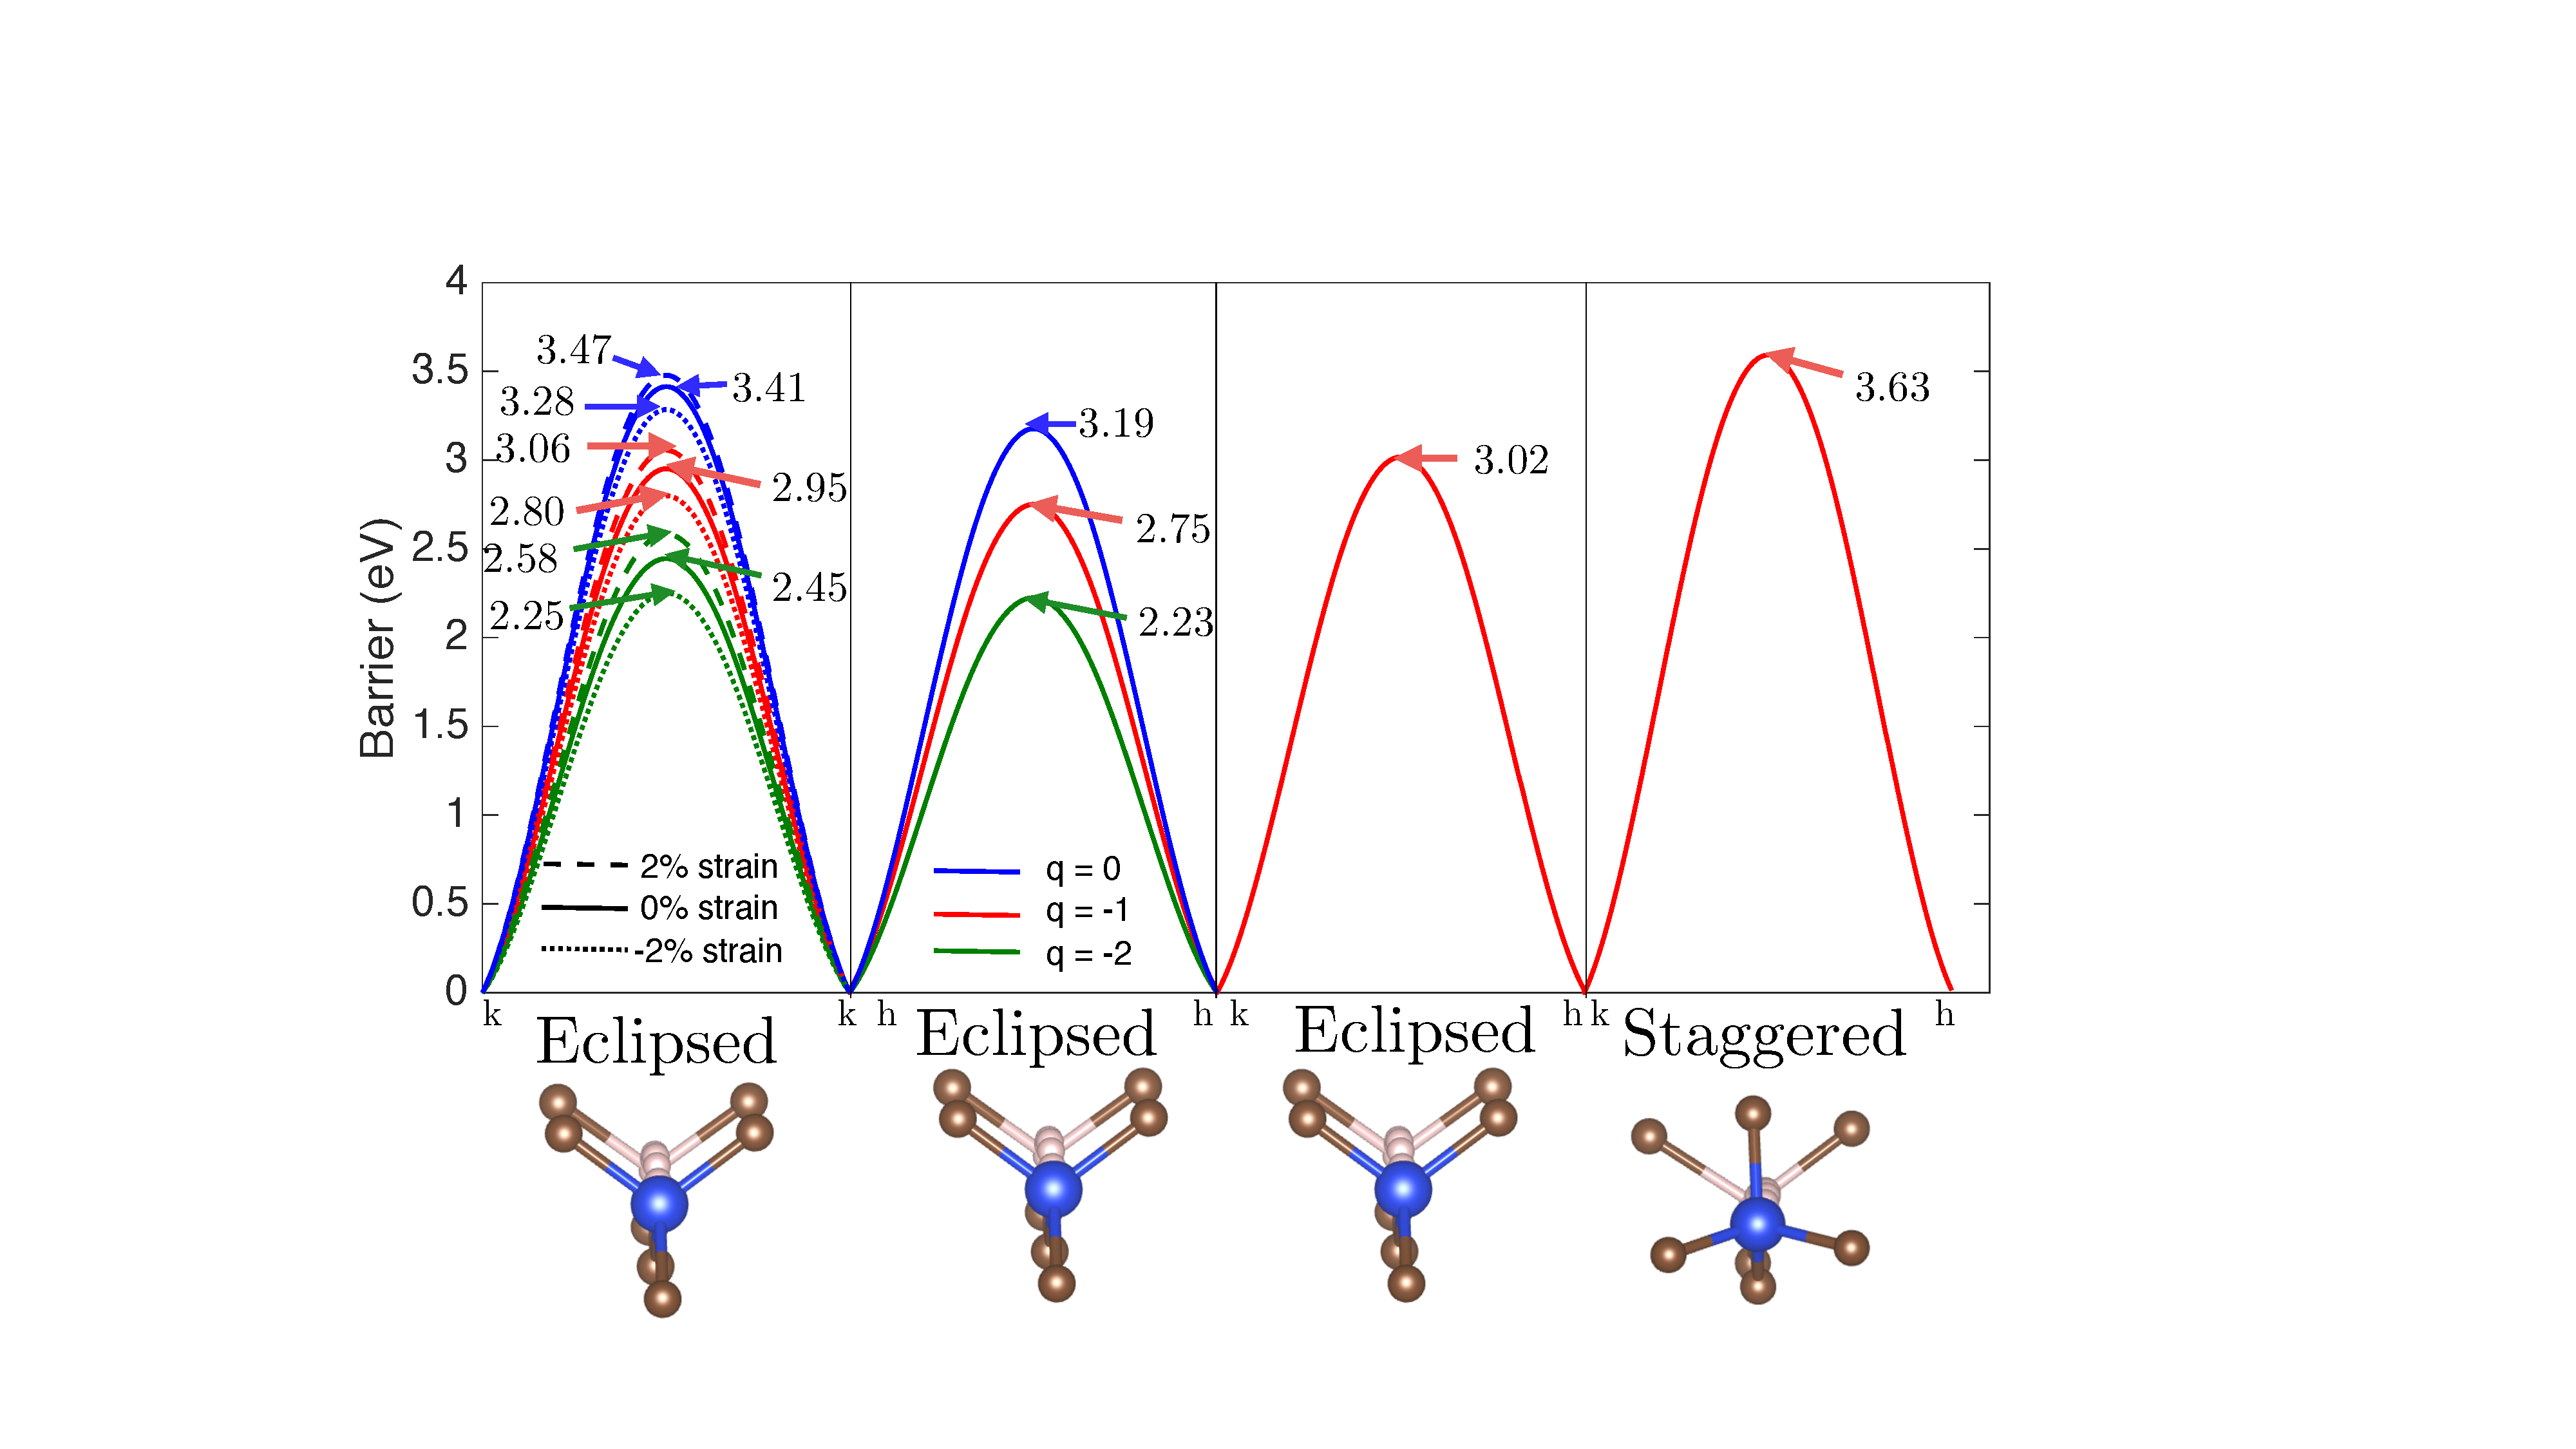
\includegraphics[width=0.9\textwidth]{barriers3.pdf}
\caption{Relative barriers to diffusion taking the starting point of diffusion between sites ($h$ or $k$ for various charge states and various strains) as the zero.} 
\label{fig:barr3}
\end{figure}

 
\section{\label{diffusivity}TRANSITION RATES}

The formula for the transition rate is,

\begin{equation}
r = \nu_0e^{-\varepsilon_b/k_BT}
\label{eq:diffusivity}
\end{equation}
where $\nu_0$ = 1.6$\times10^{13}$~s$^{-1}$, $\varepsilon_b$ is the energy barrier to diffusion and we take $T = 1300$~K. 

\section{\label{diffusivity}Approach}
Given the nature of the 4H-SiC crystal, there are 12 possible transitions - 3 transitions out of plane in the upwards direction, 3 transitions out of plane in the downwards direction, and 6 transitions in the plane. At any given time step, any one of these transitions is possible (with varying probabilities), so the problem at first pass grows as $12^N$, where $N$ is the number of time steps. More precisely, positions in 3 dimensions must be computed at each time step, the time must be updated and the probability must be updated for a total of 5 computations for each of the 12 transitions, we must then communicate the results of these 5 computations to the next processor, which will use the calculated values as inputs for an additional 5 units of work for every 12 transitions. Summing the geometric sequence corresponding to the total number of transitions at $0, 1, ..., N$ time steps, we obtain $\frac{12^{N+1}-1}{11}$, so we are dealing with a problem of size $10\cdot\frac{12^{N+1}-1}{11}$, yielding a computational complexity of $O(12^{N+1})$. We use a set of rotation matrices as a simplification in order to calculate movement in any of the in-plane and out of plane directions. Essentially, any given in-plane transition of the six, treating the current position as the origin, can be mapped onto any other in-plane transition of the six by simply rotating the original transition, in-plane, by some multiple of 60 degrees. Similarly, any upwards (downwards) transition can be mapped onto any other upwards (downwards) transition of the three by simply rotating the original transition by some multiple of 120 degrees. Thus, we define three transitions (one in-plane and two out of the plane) and obtain the remaining transitions by using rotation matrices.

Past this point, we fill a matrix $A$ with values corresponding to the $x$, $y$ and $z$ position shifts for a particular transition, the probability of transitioning, and the time shift for the particular transition. From here, we run a breadth-first search (BFS) through the tree with each node corresponding to a particular sequence of transitions, with corresponding particular final $x$, $y$ and $z$ positions and a given final or total time up to that point and a given final or total probability up to that point. There are $N$ layers to this tree and each layer has $12^N$ nodes (for a total of $\frac{12^{N+1}-1}{11}$ nodes in the tree).

Finally, we print out the $x$, $y$ and $z$ coordinates, the probability of transitioning to that a given location, and the time passed.
%\begin{figure}[ht!] 
%\centering         
%\includegraphics[width=0.45\textwidth]{T_rate3.pdf}\\
%\includegraphics[width=0.45\textwidth]{T_rate4.pdf}
%\includegraphics[width=0.45\textwidth]{T_rate5.pdf}
%\includegraphics[width=0.45\textwidth]{T_rate6.pdf}
%\includegraphics[width=0.45\textwidth]{T_rate7.pdf}
%\caption{The top figure shows effective transition rates for conversion of $k$-V$_{\rm Si}^q$ to $hk$-{V$_{\rm C}$C$_{\rm Si}$}$^q$ as a function of temperature for a value of the Fermi level corresponding to the right edge of the V$_{\rm Si}^-$ portion of the phase diagram in Fig. \ref{fig:E_form}. The bottom figures show the ratio of the transition rate for each of the four paths for diffusion of silicon vacancies to the maximum rate shown in the top figure. The calculations all seem to suggest that lower temperature would lead to lower vacancy losses.} 
%\label{fig:T_rates2}
%\end{figure}
\clearpage

\bigskip

{\bf ACKNOWLEDGMENTS:}




\bibliography{refs_SiC}
\bibliographystyle{ieeetr}

\end{document}